\documentclass[12pt,a4paper]{article}

%%% src settings
\usepackage[T2A]{fontenc}   % internal font encoding
\usepackage[utf8x]{inputenc} % text encoding 
\usepackage[russian]{babel} % document language specifics

%%% output geometry
\usepackage{geometry}
\geometry{left=2.5cm}
\geometry{right=2cm}
\geometry{top=2cm}
\geometry{bottom=2cm}

%%% math packages
\usepackage{amsmath}
\usepackage{amsfonts}
\usepackage{amssymb}

%%% listings settings
\usepackage{listings}
\lstset{
language=C++,
basicstyle=\footnotesize,       % the size of the fonts that are used for the code
numbers=left,                   % where to put the line-numbers
numberstyle=\scriptsize,        % the size of the fonts that are used for the line-numbers
stepnumber=1,                   % the step between two line-numbers. If it's 1 each line will be numbered
numbersep=5pt,                  % how far the line-numbers are from the code
backgroundcolor=\color{white},  % choose the background color. You must add \usepackage{color}
showspaces=false,               % show spaces adding particular underscores
showstringspaces=false,         % underline spaces within strings
showtabs=false,                 % show tabs within strings adding particular underscores
frame=single,	                % adds a frame around the code
tabsize=4,	                    % sets default tabsize to 4 spaces
captionpos=t,                   % sets the caption-position to bottom
breaklines=true,                % sets automatic line breaking
breakatwhitespace=false,        % sets if automatic breaks should only happen at whitespace
%inputencoding=utf8/cp1251,
morekeywords={begin,declare,fetch,close,open,while,if,for},
}
\def\lstlistingname{\large Листинг}    % listings naming

%%% figures and tables captions
\makeatletter
\renewcommand{\fnum@figure}[1]{\large Рисунок ~\thefigure{} ---}
\renewcommand{\fnum@table}[1]{\large Таблица ~\thetable{} ---}
\makeatother

%%% text options
\usepackage{pscyr} % nice cyrillic fonts
\setlength{\parindent}{1.25cm}
\usepackage{indentfirst} % paragraph indentation
\usepackage{graphicx}
\usepackage{color}
\renewcommand{\arraystretch}{1.5} % tabular cell height factor

\usepackage{sectsty}
\sectionfont{\centering}


% tables
\usepackage{subfigure}
\usepackage{tabularx}
\usepackage{multirow}
\usepackage{float}

\usepackage[page,figure,section]{totalcount}

% enumeration
\usepackage{enumitem}
\setlist{label=\arabic*), itemsep=0cm, topsep=0cm, leftmargin=1.8cm }

%%% headings and footers
\usepackage{fancyhdr}
\pagestyle{fancy}
\lhead{}
\chead{}
\rhead{\thepage}
\lfoot{}
\cfoot{}
\rfoot{}
\renewcommand{\headrulewidth}{0pt}

% reference list
\addto\captionsrussian{\def\refname{\centerline{ПЕРЕЧЕНЬ ССЫЛОК}}}

\usepackage{appendix}
%\renewcommand{\appendixtocname}{ПРИЛОЖЕНИЯ}
%\renewcommand{\appendixpagename}{\centering \LARGE ПРИЛОЖЕНИЯ}

\usepackage[unicode,pdftex]{hyperref} % make hyper refs in pdf

% типа гост блеать
\renewcommand{\rmdefault}{ftm} % Times New Roman нахуй
\allsectionsfont{\normalfont\large} % типа не жирные заголовки
\sectionfont{\centering\normalfont\large}
\subsectionfont{\indent\normalfont}

\linespread{1.2} % 1.3 типа полуторный  интервал

\makeatletter
     \renewcommand*\l@section{\@dottedtocline{1}{0em}{1.8em}}
     \renewcommand*\l@subsection{\@dottedtocline{2}{1.5em}{2.0em}}
     \renewcommand*\l@subsubsection{\@dottedtocline{3}{4.3em}{3.0em}}
\makeatother

\begin{document}

% tables numbering
\numberwithin{table}{section}
% figures numbering
\numberwithin{figure}{section}
% listings numbering
\renewcommand*{\thelstlisting}{\arabic{section}.\arabic{lstlisting}}
\makeatletter \@addtoreset{lstlisting}{section} \makeatother

%%% document structure
\setcounter{page}{3} % begin from the 3th page
\large
\begin{titlepage}

\begin{center}
Министерство образования и науки, молодежи и спорта Украины \\
Харьковский национальный университет радиоэлектроники \\

\vspace{2cm}
Факультет Компьютерной Инженерии и Управления \\
Кафедра ЭВМ

\vspace{4cm}
{\LARGE КОМПЛЕКСНЫЙ КУРСОВОЙ ПРОЕКТ} \\
ПОЯСНИТЕЛЬНАЯ ЗАПИСКА
\end{center}

\vspace{2cm}

\begin{center}
{\Large
на тему <<Разработка клавитурного тренажера>>}
\end{center}

\vspace{4cm}

{\large
\begin{tabular}{l r}
    Студент & гр. КИ-08-5 Рома~A.~C. \\
    Руководитель проекта & Аксак~Н.~Г. \\
\end{tabular}}

\vfill

\begin{center}
Харьков 2012
\end{center}

\end{titlepage}

\thispagestyle{empty}
\setcounter{page}{3}
\section*{\centering РЕФЕРАТ}

\vspace{0.6cm}
Пояснительная записка к курсовой работе содержит: \totalpages{} страниц,
\totalfigures{} рисунков, 5 ссылок и \totalsections{} приложения.

Цель исследования -- разработать законченный проект, представляющий собой
клавиатурный тренажер для слепого десятипальцевого метода набора.

Особенность разрабатываемого приложения состоит в применении кроссплатформенных
технологий, что позволит запускать приложение на всех популярных платформах.


В данном курсовом проекте в качестве технологии построения кроссплатформенных
приложений используется Qt Framework в виде привязки к языку Python(PySide),
a также базы данных SQLite.
\newline
\newline
PYTHON, PYSIDE, QT, SQLITE, GIT, ВИДЖЕТ, ТРЕНАЖЕР 


\newpage \renewcommand\thepage{}
\renewcommand\contentsname{СОДЕРЖАНИЕ \vspace{0.6cm}}
\tableofcontents
\newpage \renewcommand\thepage{\arabic{page}}


%%% document structure
\section*{\centering ВВЕДЕНИЕ}
\addcontentsline{toc}{section}{ВВЕДЕНИЕ}

\vspace{0.6cm}

В настоящее время индустрия разработки программного обеспечения переживает
бурный рост. В связи с низким порогом вхождения и количественным увеличением
числа разработчиков всё чаще возникают вопросы о качестве создаваемого программного
обеспечения.

Современный разработчик должен обладать знаниями предметной области, для которой
разрабатывается приложение, а также используемых инструментов: языка программирования,
среды разработки, отладчика, системы контроля версий и~т.~д.

На этапе принятия решения о начале разработки приложения немаловажным является
выбор используемых технологий. Правильно выбранный набор современных технологий
позволяет создавать кроссплатформенные приложения в разумные сроки.

При разработке архитектуры приложения огромное значение имеет знание и применение
разработчиком шаблонов проектирования --- известных решений проблем, часто
возникающих при разработке различных приложений.

Однако даже соблюдение рассмотренных положений само по себе не приведёт
к созданию хороших приложений. Главным остаётся наличие у разработчика
необходимого опыта использования своих знаний. Очевидное решение
данной проблемы --- участие разработчика в реальных проектах, ровно
как и создание собственных, пусть и лишь в целях обучения, а не применения
конечными пользователями.
%\section{ПОСТАНОВКА ЗАДАЧИ}
\label{sec:program}

\vspace{0.6cm}
Заданием курсового проекта является cоздание клавитурного тренажера слепого десятипальцевого метода набора.

\subsection{Описание задачи}
\label{subsec:task-description}

Разрабатываемый тренажер должен предоставлять возможность работы с несколькими пользователями. Для каждого
пользователя отдельно хранится состояние прогресса выполнения заданий. Существует возможность перепрохождения
выполненных ранее заданий.
При выполнении заданий пользователю отображается текст самого упражнения с подсветкой необходимых для набора символов.
Ошибки пользователя должны отслеживаться.Пользователю должна выводится информация о времени выполнения задания,
а также скорость печати (символы в секунду).

\section{ОБЗОР ИСПОЛЬЗУЕМЫХ ТЕХНОЛОГИЙ}
\label{sec:tech-overview}

\vspace{0.6cm}

Для реализации задачи данного курсового проекта использовались следующие
технологии:

\begin{enumerate}
    \item Git -- распределенная система контроля версий.

    \item Python -- высокоуровневый динамический язык программирования общего назначения.

    \item PySide -- кроссплатформенный инструментарий разработки ПО на языке программирования Python c использованием
          библиотеки классов Qt.

    \item SQLite -- легковесная встраиваемая реляционная база данных.

    

\end{enumerate}

\subsection{Обзор Git}
\label{subsec:git-overview}

Как уже отмечалось выше, Git -- это распределенная система управления версиями.

Система управления версиями -- это программное обеспечение для облегчения работы с
изменяющейся информацией. Система управления версиями позволяет хранить несколько версий
одного и того же документа, при необходимости возвращаться к более ранним версиям, определять,
кто и когда сделал то или иное изменение, и многое другое.

Такие системы наиболее широко используются при разработке программного обеспечения для
хранения исходных кодов разрабатываемой программы. Однако они могут с успехом применяться и
в других областях, в которых ведётся работа с большим количеством непрерывно изменяющихся электронных
документов.

Традиционные системы управления версиями используют централизованную модель, когда имеется единое
хранилище документов, управляемое специальным сервером, который и выполняет большую часть функций
по управлению версиями. Пользователь, работающий с документами, должен сначала получить нужную
ему версию документа из хранилища; обычно создаётся локальная копия документа, т. н. «рабочая копия».
Может быть получена последняя версия или любая из предыдущих, которая может быть выбрана по номеру
версии или дате создания, иногда и по другим признакам. После того, как в документ внесены нужные
изменения, новая версия помещается в хранилище. В отличие от простого сохранения файла, предыдущая
версия не стирается, а тоже остаётся в хранилище и может быть оттуда получена в любое время.

Git же напротив, использует распределенную модель. Он не нуждается в централизованном хранилище:
вся история изменения документов хранится на каждом компьютере, в локальном хранилище, и при
необходимости отдельные фрагменты истории локального хранилища синхронизируются с аналогичным хранилищем
на другом компьютере. В некоторых таких системах локальное хранилище располагается непосредственно в
каталогах рабочей копии.

Когда пользователь такой системы выполняет обычные действия, такие как извлечение определённой
версии документа, создание новой версии и тому подобное, он работает со своей локальной копией
хранилища. По мере внесения изменений, хранилища, принадлежащие разным разработчикам, начинают
различаться, и возникает необходимость в их синхронизации. Такая синхронизация может осуществляться
с помощью обмена патчами или так называемыми наборами изменений (англ. change sets) между
пользователями.

Описанная модель логически близка созданию отдельной ветки для каждого разработчика в классической
системе управления версиями (в некоторых распределённых системах перед началом работы с локальным
хранилищем нужно создать новую ветвь). Отличие состоит в том, что до момента синхронизации другие
разработчики этой ветви не видят. Пока разработчик изменяет только свою ветвь, его работа не влияет
на других участников проекта и наоборот. По завершении обособленной части работы, внесённые в ветви
изменения сливают с основной (общей) ветвью. Как при слиянии ветвей, так и при синхронизации разных
хранилищ возможны конфликты версий. На этот случай во всех системах предусмотрены те или иные методы
обнаружения и разрешения конфликтов слияния.

С точки зрения пользователя распределённая система отличается необходимостью создавать локальный
репозиторий и наличием в командном языке двух дополнительных команд: команды получения репозитория
от удалённого компьютера (pull) и передачи своего репозитория на удалённый компьютер (push). Первая
команда выполняет слияние изменений удалённого и локального репозиториев с помещением результата в
локальный репозиторий; вторая — наоборот, выполняет слияние изменений двух репозиториев с помещением
результата в удалённый репозиторий. Как правило, команды слияния в распределённых системах позволяют
выбрать, какие наборы изменений будут передаваться в другой репозиторий или извлекаться из него,
исправлять конфликты слияния непосредственно в ходе операции или после её неудачного завершения,
повторять или возобновлять неоконченное слияние. Обычно передача своих изменений в чужой репозиторий
(push) завершается удачно только при условии отсутствия конфликтов. Если конфликты возникают, пользователь
должен сначала слить версии в своём репозитории (выполнить pull), и лишь затем передавать их другим.

Основные преимущества распределённых систем -- их гибкость и значительно большая (по сравнению с
централизованными системами) автономия отдельного рабочего места. Каждый компьютер разработчика
является, фактически, самостоятельным и полнофункциональным сервером, из таких компьютеров можно
построить произвольную по структуре и уровню сложности систему, задав (как техническими, так и
административными мерами) желаемый порядок синхронизации. При этом каждый разработчик может вести
работу независимо, так, как ему удобно, изменяя и сохраняя промежуточные версии документов,
пользуясь всеми возможностями системы (в том числе доступом к истории изменений) даже в отсутствие
сетевого соединения с сервером. Связь с сервером или другими разработчиками требуется исключительно
для проведения синхронизации, при этом обмен наборами изменений может осуществляться по различным
схемам.

Ядро Git представляет собой набор утилит командной строки с параметрами. Все настройки хранятся в текстовых файлах конфигурации. Такая реализация делает Git легко портируемым на любую платформу и даёт возможность легко интегрировать Git в другие системы (в частности, создавать графические git-клиенты с любым желаемым интерфейсом).

Репозиторий Git представляет собой каталог файловой системы, в котором находятся файлы конфигурации репозитория, файлы журналов, хранящие операции, выполняемые над репозиторием, индекс, описывающий расположение файлов и хранилище, содержащее собственно файлы. Структура хранилища файлов не отражает реальную структуру хранящегося в репозитории файлового дерева, она ориентирована на повышение скорости выполнения операций с репозиторием. Когда ядро обрабатывает команду изменения (неважно, при локальных изменениях или при получении патча от другого узла), оно создаёт в хранилище новые файлы, соответствующие новым состояниям изменённых файлов. Существенно, что никакие операции не изменяют содержимого уже существующих в хранилище файлов.

\begin{figure}[h!]
    \centering
    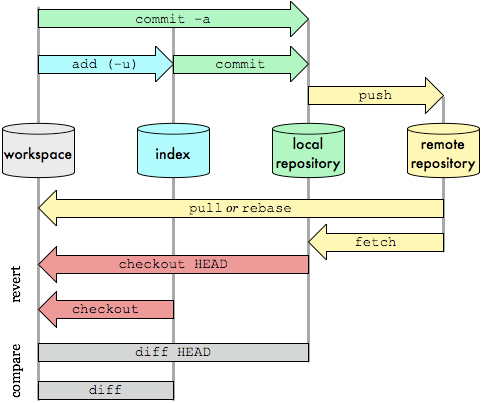
\includegraphics[scale=0.7]{images/git-overview.png}
    \caption{Процесс взаимодействия с Git}
    \label{fig:git-overview}
\end{figure}

Процесс взаимодействия с Git отображен на рисунке \ref{fig:git-overview}.

\subsection{Обзор Python}
\label{subsec:python-overview}

В связи с наблюдаемым в настоящее время стремительным развитием персональной вычислительной техники, происходит постепенное изменение требований,
предъявляемых к языкам программирования. Все большую роль начинают играть интерпретируемые языки, поскольку возрастающая мощь персональных компьютеров
начинает обеспечивать достаточную скорость выполнения интерпретируемых программ. А единственным существенным преимуществом компилируемых языков программирования
является создаваемый ими высокоскоростной код. Когда скорость выполнения программы не является критичной величиной, наиболее правильным выбором будет 
интерпретируемый язык, как более простой и гибкий инструмент программирования.

В связи с этим, определенный интерес представляет рассмотрение сравнительно нового языка программирования Python (пайтон),
который был создан его автором Гвидо ван Россумом (Guido van Rossum) в начале 90-х годов.

Python является интерпретируемым, изначально объектно-ориентированным языком программирования. Он чрезвычайно прост и содержит небольшое число ключевых слов, вместе с тем очень гибок и выразителен. Это язык более высокого уровня нежели Pascal, C++ и, естественно C,
что достигается, в основном, за счет встроенных высокоуровневых структур данных (списки, словари, тьюплы).

Несомненным достоинством является то, что интерпретатор Python реализован практически на всех платформах и операционных системах.
Первым таким языком был C, однако его типы данных на разных машинах могли занимать разное количество памяти и это служило некоторым
препятствием при написании действительно переносимой программы. Python же таким недостатком не обладает.

Следующая немаловажная черта - расширяемость языка, этому придается большое значение и, как пишет сам автор, язык был задуман именно как расширяемый.
Это означает, что имеется возможность совершенствования языка всеми всеми заинтересованными программистами. Интерпретатор написан на С и исходный код 
доступен для любых манипуляций. В случае необходимости, можно вставить его в свою программу и использовать как встроенную оболочку. Или же, написав на 
C свои дополнения к Python и скомпилировав программу, получить "расширенный" интерпретатор с новыми возможностями.

Следующее достоинство - наличие большого числа подключаемых к программе модулей, обеспечивающих различные дополнительные возможности. Такие модули пишутся на
С и на самом Python и могут быть разработаны всеми достаточно квалифицированными программистами.

Единственным недостатком, замеченным автором, является сравнительно невысокая скорость выполнения Python-программы, что обусловлено ее интерпретируемостью.
Однако, на наш взгляд, это с лихвой окупается достоинствами языка при написании программ не очень критичных к скорости выполнения. 

Python, в отличие от многих языков (Pascal, C++, Java, и т.д.), не требует описания переменных. Они создаются в месте их инициализации, т.е. 
при первом присваивании переменной какого-либо значения. Значит, тип переменной определяется типом присваиваемого значения. В этом отношении Python напоминает Basic. 
Тип переменной не является неизменным. Любое присваивание для нее корректно и это приводит лишь к тому, что типом переменной становится тип нового присваиваемого значения.

В таких языках как Pascal, C, C++ организация списков представляла некоторые трудности. Для их реализации приходилось хорошо изучать принципы работы с указателями и динамической памятью. И даже имея хорошую квалификацию, программист, каждый раз заново реализуя механизмы создания, работы и уничтожения списков, мог легко допустить трудноуловимые ошибки.
Ввиду этого были созданы некоторые средства для работы со списками. Например, в Delphi Pascal имеется класс TList, реализующий списки; для С++ 
разработана библиотека STL (Standard Template Library), содержащая такие структуры как векторы, списки, множества, словари, стеки и очереди. Однако, такие средства имеются не во всех языках и их реализациях.

Python в отличие от Pascal, C, C++ не поддерживает работу с указателями, динамической памятью и адресную арифметику. В этом он похож на Java. Как известно, указатели служат источником трудноуловимых ошибок и работа с ними относится больше к программированию на низком уровне.
Для обеспечения большей надежности и простоты они небыли включены в Python.

\subsection{Обзор PySide}
\label{subsec:qt-overview}

PySide — привязка языка Python к инструментарию Qt, совместимая на уровне API с PyQt.
В отличие от PyQt, PySide доступна для свободного использования как в открытых, так и закрытых, в частности, коммерческих, 
проектах, поскольку лицензирована по LGPL.

В свою очередь, Qt -- это кроссплатформенная библиотека для разработки ПО (изначально на С++, потом была добавленна
привязка к другим популярным языкам программирования, в частности к Python), 
разрабатываемая для написания кроссплатформенных графических приложений.

Позволяет запускать написанное с его помощью ПО в большинстве современных 
операционных систем путём простой компиляции программы для каждой ОС без 
изменения исходного кода. Включает в себя все основные классы, которые могут 
потребоваться при разработке прикладного программного обеспечения, начиная от 
элементов графического интерфейса и заканчивая классами для работы с сетью, 
базами данных и XML. Qt является полностью объектно-ориентированным, легко 
расширяемым и поддерживающим технику компонентного программирования.

Существуют версии библиотеки для Microsoft Windows, систем класса UNIX с 
графической подсистемой X11, Mac OS X, Microsoft Windows CE, встраиваемых 
Linux-систем и платформы S60. Также идёт портирование на HaikuOS, iOS, Android.

До недавнего времени библиотека Qt также распространялась ещё в одной версии: 
Qt/Embedded. Теперь эта платформа переименована в Qtopia Core и распространяется 
как отдельный продукт. Qtopia Core обеспечивает базовую функциональность для 
всей линейки платформ, предназначенных для разработки приложений для встраиваемых и 
мобильных устройств (КПК, смартфонов и т. п.).

Начиная с версии 4.5 Qt распространяется по 3 лицензиям:

\begin{enumerate}[label=--]
    \item Qt Commercial -- для разработки ПО с собственнической лицензией, 
          допускающая модификацию самой Qt без раскрытия изменений.
    \item GNU GPL -- для разработки ПО с открытыми исходниками распространяемыми 
          на условиях GNU GPL.
    \item GNU LGPL -- для разработки ПО с собственнической лицензией, но без 
          внесения изменений в Qt.
\end{enumerate}

Со времени своего появления в 1996 году библиотека Qt легла в основу тысяч 
успешных проектов во всём мире. Кроме того, Qt является фундаментом популярной 
рабочей среды KDE, входящей в состав многих дистрибутивов Linux.

Отличительная особенность Qt от других библиотек — использование
Meta Object Compiler (MOC) - предварительной системы обработки исходного кода
(в общем-то, Qt - это библиотека не для чистого C++, а для его особого наречия,
с которого и «переводит» MOC для последующей компиляции любым стандартным C++
компилятором). MOC позволяет во много раз увеличить мощь библиотек, вводя такие
понятия, как слоты и сигналы. Кроме того, это позволяет сделать код более
лаконичным. Утилита MOC ищет в заголовочных файлах на C++ описания классов,
содержащие макрос Q\_OBJECT, и создаёт дополнительный исходный файл на C++,
содержащий мета-объектный код.

Qt позволяет создавать собственные плагины и размещать их непосредственно в
панели визуального редактора. Также существует возможность расширения привычной
функциональности виджетов, связанной с размещением их на экране, отображением,
перерисовкой при изменении размеров окна.

Qt комплектуется визуальной средой разработки графического интерфейса
<<Qt Designer>>, позволяющей создавать диалоги и формы <<мышью>>
(в режиме WYSIWYG). В поставке Qt есть <<Qt Linguist>> - графическая утилита,
позволяющая упростить локализацию и перевод вашей программы на многие языки;
и «Qt Assistant» — справочная система Qt, упрощающая работу с документацией по
библиотеке, а также позволяющая создавать кросс-платформенную справку для
разрабатываемого на основе Qt ПО. Начиная с версии 4.5.0 в комплект Qt
включена среда разработки <<Qt Creator>>, которая включает в себя редактор кода,
справку, графические средства <<Qt Designer>> и возможность отладки
приложений. <<Qt Creator>> может использовать GCC или Microsoft VC++ в качестве
компилятора и GDB в качестве отладчика. Для Windows версий библиотека
комплектуется компилятором, заголовочными и объектными файлами MinGW.

Иерархия основных модулей Qt приведена на рисунке \ref{fig:qt-overview}.

\begin{figure}[h!]
    \centering
    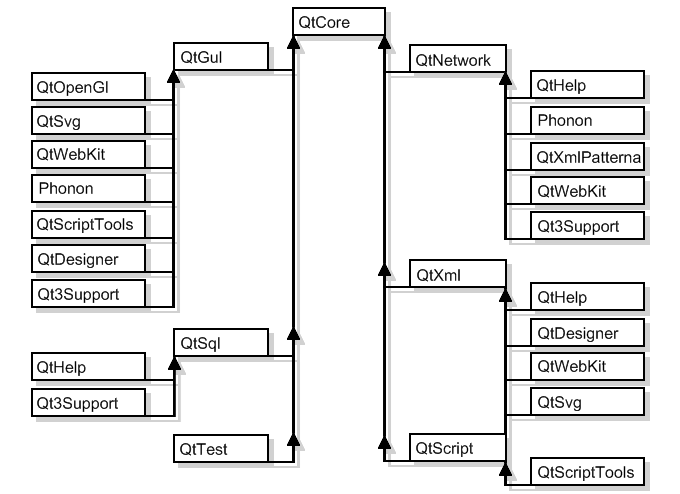
\includegraphics[scale=0.5]{images/qt-overview.png}
    \caption{Иерархия модулей Qt}
    \label{fig:qt-overview}
\end{figure}

\subsection{Обзор SQLite}
\label{subsec:sqlite-overview}

SQLite — легковесная встраиваемая реляционная база данных. Исходный код библиотеки передан в общественное достояние.
Слово «встраиваемый» означает, что SQLite не использует парадигму клиент-сервер, то есть движок SQLite не является отдельно
работающим процессом, с которым взаимодействует программа, а предоставляет библиотеку, с которой программа компонуется и движок 
становится составной частью программы. Таким образом, в качестве протокола обмена используются вызовы функций (API) библиотеки
SQLite. Такой подход уменьшает накладные расходы, время отклика и упрощает программу. SQLite хранит всю базу данных 
(включая определения, таблицы, индексы и данные) в единственном стандартном файле на том компьютере, на котором исполняется
программа. Простота реализации достигается за счёт того, что перед началом исполнения транзакции записи весь файл, хранящий 
базу данных, блокируется; ACID-функции достигаются в том числе за счёт создания файла журнала.
Несколько процессов или потоков могут одновременно без каких-либо проблем читать данные из одной базы. 
Запись в базу можно осуществить только в том случае, если никаких других запросов в данный момент не обслуживается; 
в противном случае попытка записи оканчивается неудачей, и в программу возвращается код ошибки. 
Другим вариантом развития событий является автоматическое повторение попыток записи в течение заданного интервала времени.
В комплекте поставки идёт также функциональная клиентская часть в виде исполняемого файла sqlite3, с помощью которого
демонстрируется реализация функций основной библиотеки. Клиентская часть работает из командной строки, позволяет обращаться
к файлу БД на основе типовых функций ОС.
Благодаря архитектуре движка возможно использовать SQLite как на встраиваемых системах, так и на выделенных машинах
с гигабайтными массивами данных.

Старые версии SQLite были спроектированы без каких-либо ограничений, единственным условием было то, чтобы база данных
умещалась в памяти, в которой все вычисления производились при помощи 32-разрядных целых чисел. Это создавало определённые проблемы.
Из-за того, что верхние пределы не были определены и соответственно
должным образом протестированы, то частенько наружу вылезали ошибки при использовании SQLite в достаточно экстремальных условиях.
И поэтому, в новых версиях SQLite были введены пределы, которые теперь проверяются вместе с общим набором тестов.

Сама библиотека SQLite написана на C; существует большое количество привязок к другим языкам программирования, в том числе C++, Java, VB.NET, Python, Perl, PHP, Tcl (средства для работы с Tcl включены в комплект поставки SQLite), Ruby, Haskell, Scheme, Smalltalk, Lua и Parser, а также ко многим другим. Полный список существующих средств размещён на странице проекта[3].
Простота и удобство встраивания SQLite привели к тому, что библиотека используется в браузерах, музыкальных плеерах и многих других программах.
В частности, SQLite используют:

\begin{enumerate}[label=--]
    \item Adobe Integrated Runtime — среда для запуска приложений (частично);
    \item Gears;
    \item Фреймворк Qt;
    \item Платформа XUL на движке Gecko 1.9, XULRunner 1.9 и, потенциально, все приложения, основанные на этой
          платформе, в том числе Mozilla Firefox (начиная с версии 3.0) и Mozilla Thunderbird (начиная с версии 3.0). В
          качестве примеров XUL-приложений можно привести Songbird и SQLite Manager; 
    \item Skype; 
    \item Некоторые модели GPS-навигаторов Garmin;
    \item Android API;
\end{enumerate}

Многие программы поддерживают SQLite в качестве формата хранения данных (особенно в Mac OS и iPhone OS, Android), в том
числе:

\begin{enumerate}[label=--]
    \item 1С:Предприятие 7.7 (с помощью внешнего компонента);
    \item Adobe Photoshop Lightroom;
    \item FlylinkDC++;
    \item AIMP;
    \item Banshee;
    \item Eserv;
    \item FAR Manager (начиная с версии 3.0);
    \item Gajim;
    \item Google Chrome;
    \item Miranda IM (с помощью плагина драйвера базы данных);
\end{enumerate}

В 2005 году проект получил награду Google-O’Reilly Open Source Awards.

\section{ПРОГРАММНАЯ РЕАЛИЗАЦИЯ}
\label{sec:program-implementation}

\vspace{0.6cm}

Как уже отмечалось выше, данное приложение создано при помощи динамического скриптового языка общего назначения 
Python с использованием PySide -- привязки библиотеки классов Qt к Python.

Так как при разработке данного приложения также проводилась работа с базой данных, то программная реализация будет
рассмотрена в контексте двух аспектов: основная логика работы приложения и работа с БД.

\subsection{Основная логика}
\label{sec:main}

Программа представляет собой набор виджетов -- базовых элементов для построения графического интерфейса в библитеке
Qt, в данном случае каждое отдельно окно программы является также отдельным виджетом.

Для организации взаимодействия между виджетами (переход от окна регистрации к полю выбора упражнения; запуск решения
тренажера и т.д.) был создан класс, реализующий логику управления отображением виджетов. Код данного класса приведен
в листинге \ref{lst:mainwindow}.

\lstinputlisting[language=Python, caption=Класс управления отображением, label=lst:mainwindow]{src/mainwindow.py}

Данный класс содержит поле типа QStackedWidget, которое является в некотором роде контейнером для виджетов. Обьект 
класса QStackedWidget имеет методы для добавления виджета в коллекцию, а также для доступа к определенному элементу
этой структуры.

Основной алгоритм работы следующий: все видимые виджеты должны хранить ссылку на обьект класса управления; при 
определенных действиях, когда необходимо отобразить следующее окно, виджет обращается к полю MainWindow.stack и 
добавляет в него требуемый элемент интерфейса, передавая в него ссылку на класс управления и вызывая 
методы для отображения и прорисовки. Взаимодействие между виджетами приложения строится путем использования слотов и 
сигналов -- прогрессивной технологии управления поведением программы, которая заменяет устаревающую концепцию обработки
сообщений.

Основным с точки зрения функционального назначения приложения является виджет код которого приведен в листинге \ref{lst:trainer}.

\lstinputlisting[language=Python, caption=Вид окна тренажера, label=lst:trainer]{src/trainwindow.py}

Логика построения данного класса следующая: внутри себя класс содержит два поля типа QTextEdit; одно из них является нередактируемым
и предназначено для вывода содержимого упражнения и отслеживания текущей позиции курсора, другое текстовое
поле принимает ввод пользователя с клавиатуры; логикy проверки на правильность введения следующего символа принимает на
себя перегруженный метод QTextEdit.keyPressEvent. Также в этом классе выполняется подсветка курсора в тексте упражнения,
а также подсчет времени и скорости набора (символов в секунду).

Вид окна данного виджета приведен на рисунке \ref{fig:trainer}

\begin{figure}[h!]
    \centering
    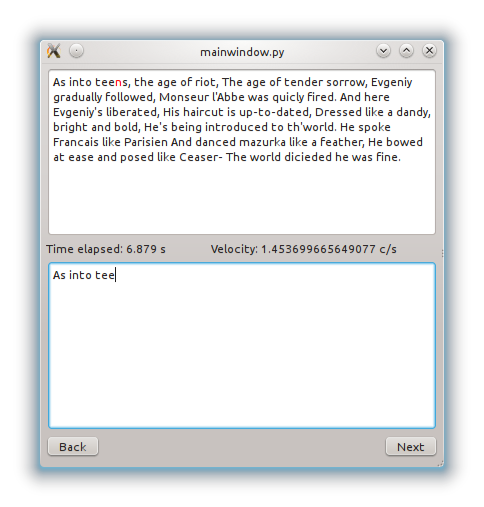
\includegraphics[scale=0.5]{images/trainer.png}
    \caption{Вид окна тренажера}
    \label{fig:trainer}
\end{figure}

Листинги кода всех виджетов приведены в приложении А.

\subsection{Работа с базой данных}
\label{sec:db}

Как уже неоднократно выше упоминалось, данное приложение в качестве базы данных использует SQLite 3-й версии.

Схема разработанной базы данных приведена на рисунке \ref{fig:db}

\begin{figure}[h!]
    \centering
    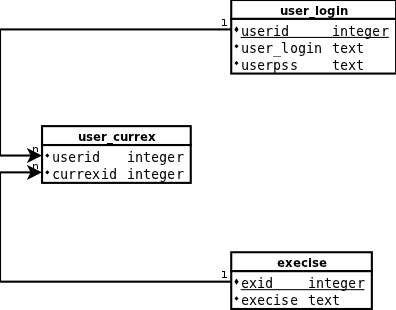
\includegraphics[scale=0.5]{images/db.png}
    \caption{Схема базы данных}
    \label{fig:db}
\end{figure}

Схема базы данных достаточно проста: хранению подлежит информация о текущем пользователе (логин и пароль), 
а также текст упражнений. Необходимо также ввести промежуточную таблицу, что обеспечивает решение проблемы 
связности, присущей всем sql-подобным базам данных.

Для взаимодействия с разработанной базой данных был создан специальный класс, который реализует концепцию DAO.
Также при проектировании данного класса был задействован паттерн Singleton. Методы класса предоставляют доступ
к информации, хранящейся в БД, тем самым производится отделение логики программы от используемых ею данных.

Код реализации приведен в листинге \ref{lst:dao}

\lstinputlisting[language=Python, caption=Реализация взаимодействия с базой данных, label=lst:dao]{src/mydao.py}


\section*{\centering ВЫВОДЫ}
\addcontentsline{toc}{section}{ВЫВОДЫ}

\vspace{0.6cm}

В ходе выполнения данного курсового проекта была разработана программа
клавиатурный тренажер, который направлен на освоение метода слепого десятипальцевого набора.
Данное приложение написано на динамическом скриптовом языке Python с использованием фреймоворка Qt 
(а именно его порта для вышеуказанного языка -- PySide), поэтому его можно запускать под всеми 
популярными платформами: MS Windows, GNU/Linux, а также Mac OS.

Особенность реализованного проекта заключается в кроссплатформенности, а также в повышенных 
показателях быстродействия, что достигается использованием современных технологий программирования
и проведением процесса оптимизации.

Разработанное приложение удовлетворяет всем выдвинутым критериям и полностью
реализует поставленную задачу.


\nocite*{}
\bibliographystyle{utf8gost780u}
\makeatletter
\renewcommand{\@biblabel}[1]{#1.}
\makeatother
\bibliography{lit}
\addcontentsline{toc}{section}{ПЕРЕЧЕНЬ ССЫЛОК}

%\appendix
%\appendixpage
%\addappheadtotoc

\section*{ПРИЛОЖЕНИЕ А. ЛИСТИНГ ПРОГРАММЫ ТРЕНАЖЕРА }
\addcontentsline{toc}{section}{ПРИЛОЖЕНИЕ А. ЛИСТИНГ ПРОГРАММЫ ТРЕНАЖЕРА}
\label{adx:main} 

\renewcommand*{\thelstlisting}{\arabic{lstlisting}}

\lstinputlisting[language=Python, caption=mainwindonw.py]{src/mainwindow.py}
\lstinputlisting[language=Python, caption=userchoice.py]{src/userchoice.py}
\lstinputlisting[language=Python, caption=exercises.py]{src/exersises.py}
\lstinputlisting[language=Python, caption=trainwindow.py]{src/trainwindow.py}


\newpage
\section*{ПРИЛОЖЕНИЕ Б. ЛИСТИНГ РАБОТА С БАЗОЙ ДАННЫХ}
\addcontentsline{toc}{section}{ПРИЛОЖЕНИЕ Б. ЛИСТИНГ РАБОТА С БАЗОЙ ДАННЫХ}
\label{adx:db}

\lstinputlisting[language=Python, caption=mydao.py]{src/mydao.py}



\end{document}
